\documentclass[12pt]{ctexart}
    \title{PING程序的实现}
    \author{162020321 朱家震}
    \pagestyle{empty}
    \usepackage{amsmath}
    \usepackage[a4paper,left=2.5cm,right=2.5cm,top=2cm,bottom=2cm]{geometry}
    \usepackage{amsfonts}
    \usepackage{amssymb}
    \usepackage{amsthm,amsmath}
    \usepackage{mathrsfs}
    \usepackage{indentfirst}
    \usepackage{multirow}
    \usepackage{graphicx}
    \usepackage{float}
    %\usepackage{pythonhighlight}
    \usepackage{subfigure}
    \usepackage[usenames,dvipsnames]{xcolor}
    \usepackage[ruled,linesnumbered]{algorithm2e}
    \usepackage{bm} 
    \RequirePackage{xcolor}
    \definecolor{winered}{rgb}{0.5,0,0}

    \definecolor{lightgrey}{rgb}{0.95,0.95,0.95}
    \definecolor{commentcolor}{RGB}{0,100,0}
    \definecolor{frenchplum}{RGB}{190,20,83}

    \usepackage{listings}
    \newfontfamily\courier{Courier New}
    \lstdefinestyle{estyle}{
        basicstyle=%
          \ttfamily
          \lst@ifdisplaystyle\footnotesize\fi
      }
      \lstset{basicstyle=\scriptsize\ttfamily,style=estyle}
      
      \lstset{language=[LaTeX]TeX,
          texcsstyle=*\color{winered},
          numbers=none,
          breaklines=true,
          keywordstyle=\color{winered},
          frame=tlbr,framesep=4pt,framerule=0pt,
          commentstyle=\color{commentcolor},
          emph={elegantpaper,fontenc,fontspec,xeCJK,FiraMono,xunicode,newtxmath,figure,fig,image,img,table,itemize,enumerate,newtxtext,newtxtt,ctex,microtype,description,times,newtx,booktabs,tabular,PDFLaTeX,XeLaTeX,type1cm,BibTeX,cite,gbt7714,lang},
          emphstyle={\color{frenchplum}},
          morekeywords={DeclareSymbolFont,SetSymbolFont,toprule,midrule,bottomrule,institute,version,includegraphics,setmainfont,setsansfont,setmonofont ,setCJKmainfont,setCJKsansfont,setCJKmonofont,RequirePackage,figref,tabref,email,maketitle,keywords,zhdate,zhtoday},
          tabsize=2,
          backgroundcolor=\color{lightgrey}
      }
\makeatletter %使\section中的内容左对齐
%\renewcommand{\section}{\@startsection{section}{1}{0mm}
% {-\baselineskip}{0.5\baselineskip}{\bf\leftline}}
\makeatother
%\renewcommand\thesubsectiondis{\section.\arabic{subsection}}  %重定义语句
\begin{document}
    \maketitle
    \setcounter{section}{0}
    \section{实验内容}
    \subsection{实验目的}

    理解tracert程序的概念,熟练使用原始套接字

    \subsection{实验环境}

    Linux,C

    \subsection{实验内容}

    设计一个简单的tracert程序。

    \section{实验设计}
    \subsection{程序执行}

    首先我们在Windows上执行tracert程序,了解我们要做的输出是什么样的,执行出来的效果如下:
    
    \begin{figure}[H]
        \centering
        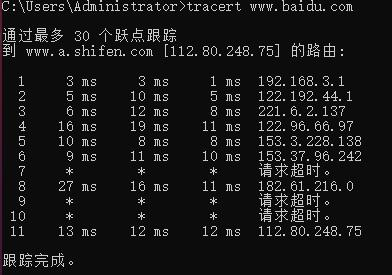
\includegraphics[width=5in]{figures/cmd.jpg}
        \label{sw}
        \caption{windows终端执行结果}
    \end{figure}

    \begin{figure}[H]
        \centering
        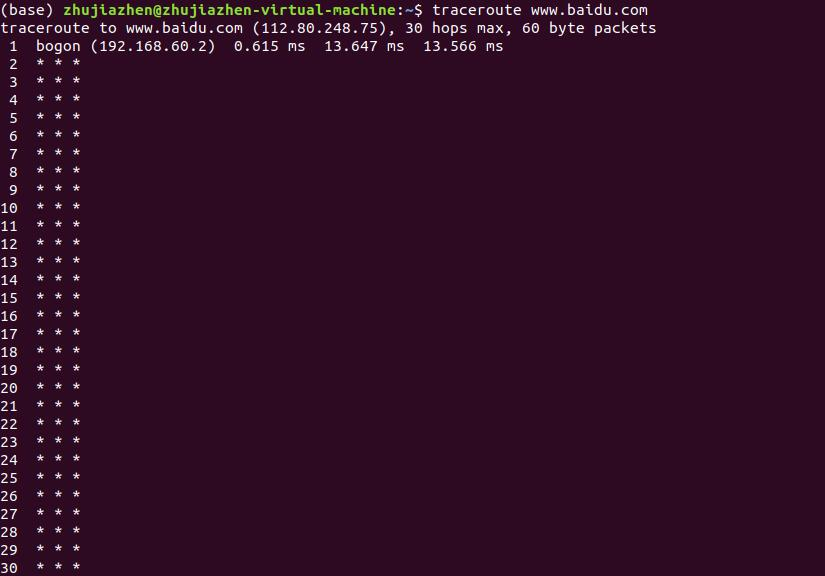
\includegraphics[width=5in]{figures/linux.jpg}
        \label{li}
        \caption{Linux终端执行结果}
    \end{figure}

    我们发现在Linux上执行的traceroute输出都是“*”,也就是超时,只能收到第一个跃点的地址。通过查询发现linux虚拟机在traceroute时,默认使用UDP报文,而不是使用ICMP报文;而防火墙为了方便网络调试是放行了ICMP报文,但没有放行UDP报文,这就导致了linux虚拟机的traceroute报文(UDP)被防火墙拦截了,windows虚拟机的traceroute报文(ICMP)正常通行。

    \begin{figure}[H]
        \centering
        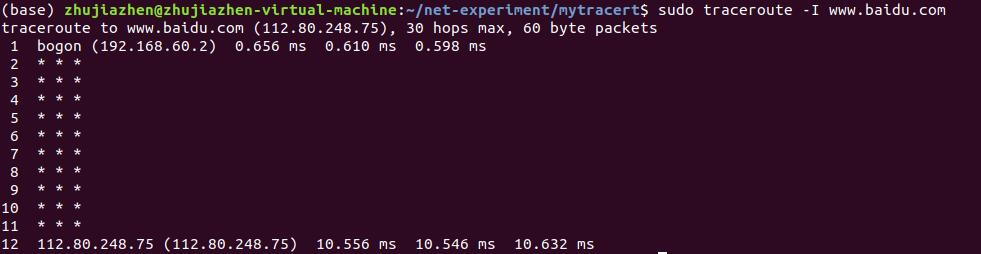
\includegraphics[width=5in]{figures/linux-true.jpg}
        \label{li2}
        \caption{Linux终端执行结果}
    \end{figure}

    当我们使用-I发送ICMP包时可以发现能够正常收回。接下来我们就根据Linux输出进行一个复现。

    \section{关键程序}
    其程序大体与myping程序类似,只需要在发送包之前设置包的ttl即可。在报告中只插入了与myping代码不同的函数,详情可以见附代码文件。

    \subsection{创建不同ttl的套接字}
    \begin{lstlisting}
int create_socket(int ttl) 
{
    int sockfd = socket(AF_INET, SOCK_RAW, IPPROTO_ICMP);
    if (sockfd < 0) {
        perror("socket error");
        return -1;
    }
    if (setsockopt(sockfd, IPPROTO_IP, IP_TTL, &ttl, sizeof(ttl)) < 0) {
        perror("setsockopt error");
        close(sockfd);
        return -1;
    }
    struct timeval timeout = {TIMEOUT, 0};
    if (setsockopt(sockfd, SOL_SOCKET, SO_RCVTIMEO, &timeout, sizeof(timeout)) < 0) {
        perror("setsockopt error");
        close(sockfd);
        return -1;
    }
    return sockfd;
}
    \end{lstlisting}

    在这里使用$setsockopt$函数设置ttl值,函数详情为:
    \begin{lstlisting}
int setsockopt(int sockfd, int level, int optname,const void *optval, socklen_t optlen);
sockfd:标识一个套接口的描述字。
level:选项定义的层次;支持SOL_SOCKET、IPPROTO_TCP、IPPROTO_IP和IPPROTO_IPV6。
optname:需设置的选项。
optval:指针,指向存放选项待设置的新值的缓冲区。
optlen:optval缓冲区长度。
    \end{lstlisting}

    \subsection{接收ICMP包}
    
    在这里接收时,我们需要处理不同的ICMP\_TYPE,根据情况是ICMP\_TIME\_EXCEEDED还是ICMP\_ECHOREPLY亦或是其他返回不同的值进行处理。

    \begin{lstlisting}
int recv_icmp_reply(int sockfd, struct sockaddr_in* from, struct timeval *start_time) 
{
    char packet[PACKET_SIZE];
    memset(packet, 0, sizeof(packet));
    socklen_t fromlen = sizeof(*from);
    struct timeval end_time;
    
    int n = recvfrom(sockfd, packet, sizeof(packet), 0, (struct sockaddr *)from, &fromlen);
    gettimeofday(&end_time, NULL);
    if (n < 0) {
        if (errno == EAGAIN || errno == EWOULDBLOCK) {
            printf(" *          ");
            return 2;
        } else {
            perror("recvfrom error");
            return -1;
        }
    }
    struct iphdr *iph = (struct iphdr *)packet;
    struct icmphdr *icmph = (struct icmphdr *)(packet + (iph->ihl << 2));
    if (icmph->type == ICMP_ECHOREPLY) {
        double elapsed_time = (end_time.tv_sec - start_time->tv_sec) * 1000.0 + (end_time.tv_usec - start_time->tv_usec) / 1000.0;
        printf(" %fms ", elapsed_time);        
        return 1;
    } else if (icmph->type == ICMP_TIME_EXCEEDED) {
        double elapsed_time = (end_time.tv_sec - start_time->tv_sec) * 1000.0 + (end_time.tv_usec - start_time->tv_usec) / 1000.0;
        printf(" %fms ", elapsed_time);
        return 0;
    } else {
        printf(" *          ");
        return -1;
    }
}
    \end{lstlisting}

    \subsection{tracert函数}

    这个函数用于实现tracert的主要功能。根据实际的运行结果可以发现每一个跃点都是发送三个数据包的,这里我也每个跃点发送三个数据包。

    \begin{lstlisting}
void tracert(const char* host) {
    struct addrinfo* res = resolve_host(host);
    if (res == NULL) {
        return;
    }
    char ipstr[INET6_ADDRSTRLEN];
    inet_ntop(res->ai_family, &((struct sockaddr_in *)res->ai_addr)->sin_addr, ipstr, sizeof(ipstr));
    printf("Tracing route to %s [%s] over a maximum of %d hops:\n", host, ipstr, MAX_HOPS);
    int ttl, seq, sockfd, done = 0;
    struct sockaddr_in addr;

    for (ttl = 1; ttl <= MAX_HOPS && !done; ttl++) {
        printf("%2d  ", ttl);
        fflush(stdout);
        for (seq = 0; seq < 3; seq++) {
            sockfd = create_socket(ttl);
            if (sockfd < 0) {
                return;
            }
            memset(&addr, 0, sizeof(addr));
            addr.sin_family = AF_INET;
            addr.sin_addr = ((struct sockaddr_in *)res->ai_addr)->sin_addr;
            addr.sin_port = htons(0);
    
            if (send_icmp_request(sockfd, &addr, seq) < 0) {
                close(sockfd);
                continue;
            }

            struct timeval tv;
            gettimeofday(&tv, NULL);
            int ret = recv_icmp_reply(sockfd, &addr, &tv);

            if (ret < 0) {
                close(sockfd);
                continue;
            }

            char ipstr1[INET6_ADDRSTRLEN];
            format_addr(&addr, ipstr1, sizeof(ipstr1));
            
            if (ret == 2) continue;
            else if (ret == 0 && seq == 2) {
                printf("%-15s", ipstr1); 
                continue;
            }
            else if (ret == 0) continue;
            else if (seq == 2) {
                if (done) {
                    printf("%-15s", ipstr1); 
                    break;
                }
                printf("\n");
                continue;
            }
            if (seq == 2)
                printf("%-15s", ipstr1); 
            if (strcmp(ipstr, ipstr1) == 0) {
                done = 1;
            }
            close(sockfd);
        }
        printf("\n");
    }
    freeaddrinfo(res);
}
\end{lstlisting}
    \section{实验结果与分析}

    最终,try3的运行结果如下图所示。

    \begin{figure}[H]
        \centering
        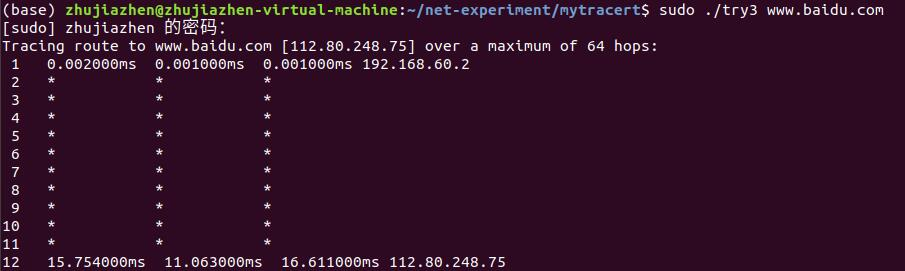
\includegraphics[width=5in]{figures/res.jpg}
        \label{rw}
        \caption{myping终端执行结果}
    \end{figure}
    
    可以看到Linux下访问百度的时候只要两跳就能到,但是Windows的cmd的tracert却要好多跳,具体原理我还不是很清楚。
    
\end{document}